%!TEX root = ../../prace.tex

\section{Počáteční inicializace projektu}

Pokud je cílem spustit projekt hry ze zdrojových kódů, je potřeba si stáhnout \UE{} ve verzi \TT{4.15.3}. Na hlavní stránce \UE{} je potřeba stáhnout \textit{Epic Games Launcher} (ke stažení zde~\citep{ue_download}). Po vytvoření uživatelského účtu a~následnému přihlášení do aplikace bude vidět obrazovka podobná obrázku \ref{fig:ueLauncher}:


\begin{figure}[!ht]\centering
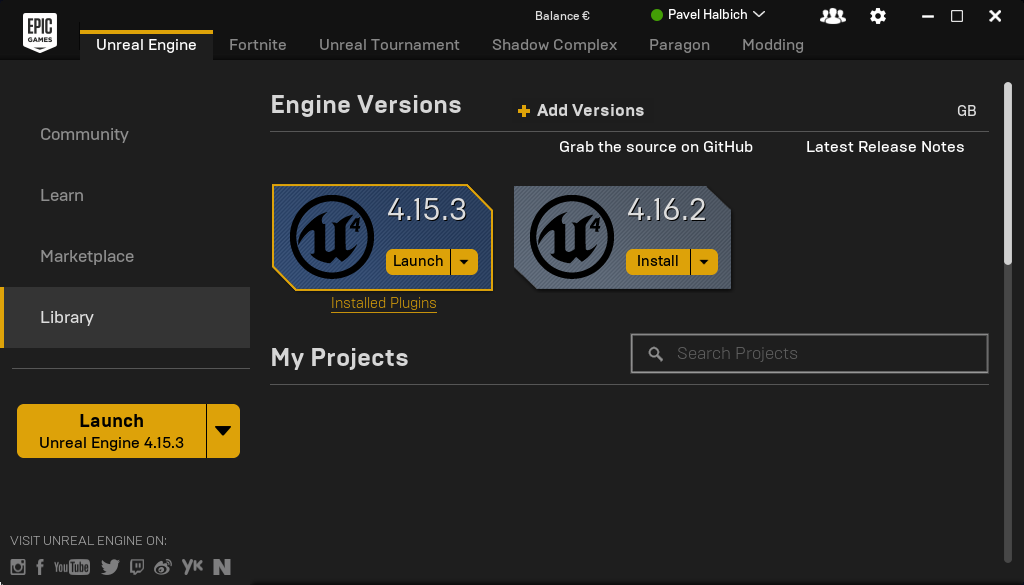
\includegraphics[ width=140mm]{../img/program/ueLauncher}

\caption{Epic Games Launcher}
\label{fig:ueLauncher}

\end{figure}

\FloatBarrier

Pokud není vidět \UE{} dané verze v~seznamu verzí, je potřeba jej přidat kliknutím na tlačítko \textit{Add Versions} a~případném následném výběru správné verze. Na obrázku \ref{fig:ueLauncher} je vidět \UE{} verze \TT{4.16.2}, který je připravený ke stažení. Posledním krokem je samotná instalace stisknutím tlačítka \textit{Install}. Použití novější verze \UEu{} je možné, ale běžnému uživateli to nedoporučujeme. Mezi verzemi se mohou projevit nekompatibility v~kódu, které je mnohdy nutné řešit zásahy přímo do zdrojových kódů hry.

TODO lépe popsat, že se vytváří VS projekt ze zdrojáků -- je to standardníá

Dále je potřeba mít k~dispozici zdrojové kódy ať už z~DVD, nebo z~tohoto release na GitHubu (odkaz~\citep{gh_finalRelease}).
 
Následujícím krokem je vytvoření projektu hry. Toho se docílí kliknutím pravým tlačítkem myši na soubor \TT{TauCetiF2.uproject} a~následnou volbou \textit{Generate Visual Studio project files} (viz obrázek \ref{fig:generateProjectFiles}). 

\begin{figure}[!ht]\centering
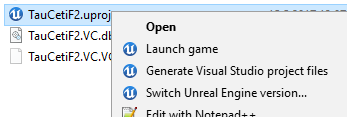
\includegraphics[ width=80mm]{../img/program/generateProjectFiles}

\caption{Vytvoření projektu hry}
\label{fig:generateProjectFiles}

\end{figure}

\FloatBarrier


Pokud v~kontextové nabídce chybí možnosti pro \UE{}, je potřeba provést asociaci s~\TT{uproject} soubory. Tato asociace by měla být provedena automaticky, nejpozději po vytvoření libovolného \CPP{} projektu z~kterékoliv šablony Ze zkušenosti autora -- toto se mnohdy nemusí podařit. Pokud se nepodaří vygenerovat projekt hry, může pomoci otevřít editor přes \textit{Epic Games Launcher}, najít a~otevřít projekt a~po načtení vybrat možnost obnovy projektu, jak je naznačeno na obrázku \ref{fig:ue_refresh}. K~tomu je zapotřebí mít Visual Studio 2015 alespoň ve verzi \textit{Community}.


\begin{figure}[!ht]\centering
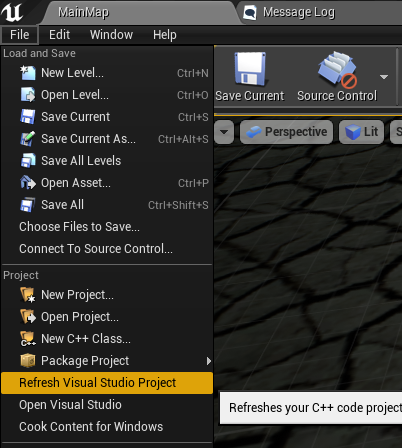
\includegraphics[ width=80mm]{../img/program/ue_refresh}

\caption{Vygenerovaný projekt hry}
\label{fig:ue_refresh}

\end{figure}

\FloatBarrier



Pokud i~toto selže, ověřte si, prosím, že je možné založit nějaký projekt založený na \CPP{}, zkompilovat jej a~taktéž vygenerovat projekt pro Visual Studio. Pokud se to povede s~projektem z~nějaké připravené šablony, mělo by to fungovat i~s~naší hrou.


Předposledním krokem je v~případě úspěšného vytvoření projektu hry jeho otevření ve \textit{Visual Studiu}, nastavení \textit{TauCetiF2} jako hlavní spustitelnou část projektu (viz obrázek \ref{fig:vs}) a~následné spuštění  editoru hry.


\begin{figure}[!ht]\centering
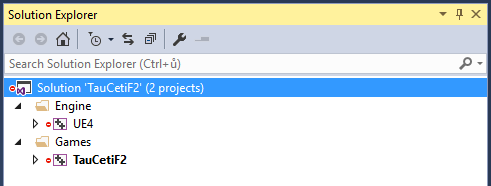
\includegraphics[ width=110mm]{../img/program/vs}

\caption{Vygenerování projektu hry}
\label{fig:vs}

\end{figure}

\FloatBarrier




